\subsection{The index of a linear mapping}

Let L be a field \(^{1}\) , let U and V be two vector spaces \(^{2}\) over L and \(f: U \to V\) an L-linear mapping; f is said to have finite index if the kernel N and cokernel C of f have finite dimension, and the integer

\[
\chi (f) = [ \mathrm{C}: \mathrm{L} ] - [ \mathrm{N}: \mathrm{L} ]
\]

is called the index of \(f\) .

Every linear mapping \(f: \mathrm{U} \to \mathrm{V}\) possesses an index equal to \([\mathrm{V}: \mathrm{L}] - [\mathrm{U}: \mathrm{L}]\) . Let \(\mathbf{N}\) be the kernel, \(\mathbf{I}\) the image and \(\mathbf{C}\) the cokernel of \(f\) . We have \(\mathbf{C} = \mathbf{V} / \mathbf{I}\) and \(\mathbf{I}\) is isomorphic to \(\mathbf{U} / \mathbf{N}\) ; thus we have \([\mathrm{U}: \mathrm{L}] = [\mathrm{N}: \mathrm{L}] + [\mathrm{I}: \mathrm{L}]\) and \([\mathrm{V}: \mathrm{L}] = [\mathrm{C}: \mathrm{L}] + [\mathrm{I}: \mathrm{L}]\) , whence the result.

Lemma 2. --- Let \(f: \mathbf{U} \to \mathbf{V}\) and \(g: \mathbf{V} \to \mathbf{W}\) be two L-linear mappings. If \(f\) and \(g\) each have an index, the same is true of \(g \circ f\) and we have

\[
\chi (g \circ f) = \chi (f) + \chi (g).
\]

Put \(h = g \circ f\) , and denote by \(\mathbf{N}, \mathbf{N}'\) , \(\mathbf{N}''\) the kernels of \(f, g, h\) respectively and by \(\mathbf{C}, \mathbf{C}'\) , \(\mathbf{C}''\) their cokernels. We have \(\mathbf{N} \subset \mathbf{N}'' \subset \mathbf{U}\) and \(f(\mathbf{N}^{\prime\prime}) = f(\mathbf{U}) \cap \mathbf{N}'\) ; hence there exists a linear mapping \(\bar{f}: \mathbf{N}^{\prime\prime} \to \mathbf{N}'\) agreeing with \(f\) on \(\mathbf{N}''\) and with kernel \(\mathbf{N}\) . The canonical mapping \(\pi\) of \(\mathbf{V}\) onto \(\mathbf{C} = \mathbf{V}/f(\mathbf{U})\) induces a mapping \(\pi'\) of \(\mathbf{N}'\) into \(\mathbf{C}\) whose kernel is \(f(\mathbf{U}) \cap \mathbf{N}' = \bar{f}(\mathbf{N}^{\prime\prime})\) . By passage to quotients \(g\) defines a mapping \(\bar{g}\) of \(\mathbf{C} = \mathbf{V}/f(\mathbf{U})\) into \(\mathbf{C}'' = \mathbf{W}/g(f(\mathbf{U}))\) whose kernel is clearly \((\mathbf{N}' + f(\mathbf{U}))/f(\mathbf{U}) = \pi'(\mathbf{N}')\) . Finally the canonical mapping \(\rho\) of \(\mathbf{C}'' = \mathbf{W}/g(f(\mathbf{U}))\) onto \(\mathbf{C}' = \mathbf{W}/g(\mathbf{V})\) has the kernel \(g(\mathbf{V})/g(f(\mathbf{U})) = \bar{g}(\mathbf{C})\) . To sum up, we have established the exactness of the sequence

\[
0 \to \mathrm{N} \stackrel {i} {\to} \mathrm{N} ^ {\prime \prime} \stackrel {\bar {f}} {\to} \mathrm{N} ^ {\prime} \stackrel {\pi^ {\prime}} {\to} \mathrm{C} \stackrel {\bar {g}} {\to} \mathrm{C} ^ {\prime \prime} \stackrel {\rho} {\to} \mathrm{C} ^ {\prime} \to 0
\]

(where \(i\) is the canonical injection of \(\mathbf{N}\) in \(\mathbf{N}''\) ).

\pandocbounded{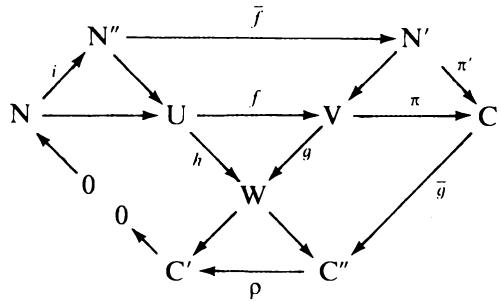
\includegraphics[keepaspectratio]{images/part002_9769358f.jpg}}\\
FIG. 1

By hypothesis N, N', C and C' are of finite dimension; hence the same is true of N'' and C''. By Cor. 2 (II, p.~295) we then have

\[
[ \mathrm{N}: \mathrm{L} ] - [ \mathrm{N} ^ {\prime \prime}: \mathrm{L} ] + [ \mathrm{N} ^ {\prime}: \mathrm{L} ] - [ \mathrm{C}: \mathrm{L} ] + [ \mathrm{C} ^ {\prime \prime}: \mathrm{L} ] - [ \mathrm{C} ^ {\prime}: \mathrm{L} ] = 0
\]

whence \(\chi(h) = \chi(f) + \chi(g)\) .

